\documentclass[../intro.tex]{subfiles}
\begin{document}
\section{Notation \& Definitions}
\begin{figure}
    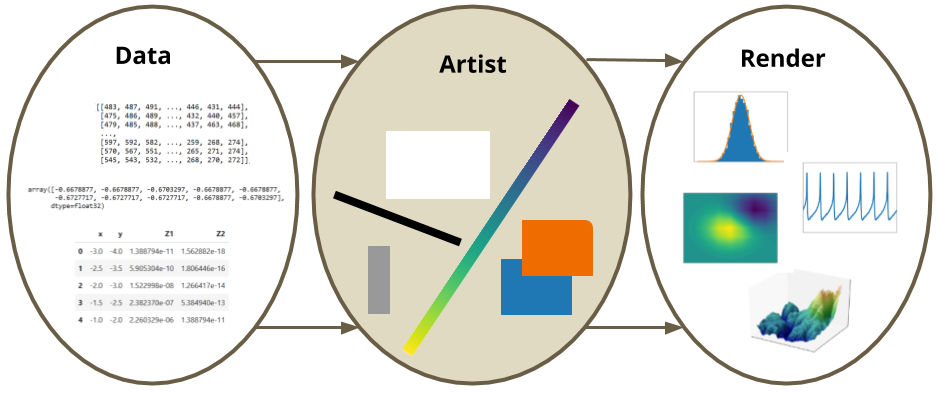
\includegraphics{figures/sections/dar.png}
    \caption{Data with semantic structure (such as tables and images) is mapped to visual encodings (color, position) that are composited into visual idioms (scatter, line) that are rendered into graphics (rasters, vectors).}
    \label{fig:artists}
\end{figure}
Figure~\ref{fig:artists} shows transformation from data into rendered graphical object, wherein there is an intermediate artist stage where the data gets transformed into a visual form. We argue that a faithful representation of the data is one where:
invariance:
functor
* types: variables measurement groups are  with visual encoding groups
* topology: visual idioms preserve the topology/connectivity of the dat


We propose that the mapping of a precise subset of data to a visual idiom ($I$) can be encapsulated in a class of functors called artists.
Gluing keys along a base space

| Fiber Bundle | Spivak |
|--------------|--------|
| B | K |
| F | U |
| embedded in F  | (C, \sigma), \pi |
| E/V |  |
|   | \tau:  K-\Gamma(sigma) |
|   |

\begin{equation}
    A: {\sigma \in \Gamma(V)}\mapsto f:\T \mapsto R^{7}
\end{equation}
diagram here: gamma is a dataframe, t is like xkcd line (clear abstract), R7 is nice pixelated version 
\begin{definition}
    \item[$F$] fiber, which is the space of all possible values encoded in the fiber bundle
    \item[$K$] base space, tells how the values in the fibers are connected, is analogous to the indexer in data containers
    \item[$V$] $F$ = $K \X F$ total space of the fiber bundle, which is space of all possible values on the index 
    \item[$\sigma(k)$] section of the fiber at a single k, (record on the  r) (dataframe)
    \item[$\Gamma(V)$] set of all possible sections (Spivak - $\Gamma(\sigma))$ - is space of all dataframes (we use this in artists to generalize- class of functions/sigmas that the artist can work on)
    \item[$f$] analogous to spec (such as svg or raster) that render will rely on to translate image to screen
    \item[$\T \in CW$] cw simplex representing topology of visual elements on screen (embedded in code rather than explicit) 
    \item[$R^{7}$]  {R,G,B,A, x, y, z} pixel in display space
\end{definition}

\begin{equation}
    A: {\sigma \in \Gamma(V)}\mapsto f:\T \mapsto R^{7}
\end{equation}

\subsubsection{Data}
We use Butler's visualization model built on the mathematics of fiber bundles \cite{butlerVectorBundleClassesForm1992,butlerVisualizationModelBased1989} and Spivak's schema like description of fibers \cite{spivakSIMPLICIALDATABASES} as the basis of our data model.  The components of the fiber bundle are:
\begin{definition}
    \item[$K$] base space that describes the topology of the data, is the indexer in data contain
\end{definition}

\begin{center}
    \begin{tabular}{ c c c }
     term & mathematical definition & data container analogue\\
      $K$ & base space along which the data lies & indexer \\
      $F$ & fiber space from which possible values are pulled & schema \\
      $E$ & trivial: $F= K \times F$, non-trivial \dots & 
      
    \end{tabular}
\end{center}


\begin{equation}

\end{equation}

\subsection{artist}
%%category theory diagrams to show artist is a functor, which is how you get invariance
%% artist is parameterized on taus
%% artists are curried collection of taus , orbits of artists are the visual idiomsW
\begin{equation}
    A: \Gamma(V), \Taus \mapsto f:\T \mapsto R^{7}
\end{equation}

%%%in practuce this has currently same topology as gamma V
\begin{equation}%%pull in spivak
    \tau: one type in the fiber \mapsto different type in the T fiber 
\begin{equation}

\subsection{render}
\begin{equation}
    f: \T \mapsto R^{7}
\end{equation}

\end{document}